
\chapter{Onderzoek: Methode extactie project dependency informatie}\label{ch:onderzoek:-methode-extactie-project-dependency-informatie}
Voordat er een ontwerp gemaakt kan worden voor de nieuwe module moet er uitgezocht worden of de data die uit de geselecteerde tools komen relevant en bruikbaar zijn. Om dit uit te zoeken wordt er een test opstelling gemaakt die het mogelijk maakt om de output te analyseren op een bestaand project. Daarnaast moet er op basis van deze gegevens worden onderzocht welke manier het beste is om de projecten vervolgens te analyseren gezien we hier kunnen kiezen om dit in de pipeline te doen of door de nieuwe module op basis van gegevens die geleverd worden door de pipeline. De hoofdvraag voor dit onderzoek is dan ook: "Welke methode is het meest efficiënt om projecten te analyseren, zonder dat de Jenkins pipeline hier invloed van ondervindt en de gegevens niet correct zijn. Deze hoofdvraag roept een aantal deelvragen op die ieders beantwoord dienen te worden:
\begin{itemize}
    \item Welke output komt er uit de gelecteerde tools en is deze bruikbaar voor het doel van de opdracht?
    \item Op welke manier kunnen de tools worden ingezet?
    \item Wat is de meeste efficiënte manier om de projecten te analyseren?
    \item Hoe wordt er gegarandeerd dat de gegevens correct zijn?
\end{itemize}
Met de resultaten kan uiteindelijk besloten worden op welk moment er een analyse gedaan wordt: Tijdens de build op de Jenkins server of op een later moment(zelfde dag) middels de API van de module.

\section{Methode}\label{sec:methode}
Om de juiste resultaten in dit onderzoek te krijgen is er gekozen om een test omgeving op te zetten waarbij een dependency analyse wordt gesimuleert. Een testomgeving bied de mogelijkheid om in een gecontroleerde situatie metingen te verichten. Te denken aan de tijd die het kost om een analyse uit te voeren op projecten van verschillende grote. Een mogelijkheid om op verschillende manieren informatie over dependencies uit projecten te verkrijgen.
\subsection{opzet testomgeving}\label{subsec:opzet-testomgeving}
Als eerste dient er een "sandbox" Scala play applicatie opgezet te worden. deze applicatie dient de volgende zaken te kunnen doen:
\begin{itemize}
    \item Meten hoelang een analyse duurt.
    \item Verschillende methoden om intern en extern een analyse te doen.
    \item Omgaan met GitLab Repo's om dan al niet de dependency info te verkrijgen of het complete project op basis van een hashcode van de commit
\end{itemize}

\subsection{}

\subsection{test projecten}
Om een beeld te verkrijgen in de verschillen in projecten moeten er meerdere projecten worden gebruikt. Dit zijn projecten die al door EagleScience worden ontwikkeld en zijn geselecteerd op basis van de hoeveelheid gebruikte externe bibliotheken.
De selectie is nu:
\begin{itemize}
    \item GroeiGids
    \item SAM
    \item PTX
\end{itemize}


\section{Hoe zijn de geselecteerde tools te implementeren, en wat is het resultaat?}
Om te kijken hoe de tools kunnen worden geimplementeerd dient er een testopstelling gebouwd worden die een bijna identieke omgeving nabootst in de projecten die geanalyseerd dienen te worden. Er worden twee projecten geselecteerd op basis van het formaat van de aantal dependencies om deze redenen kunnen we nagaan of er tijd verloren gaat in de analyse.



\begin{itemize}
    \item snelheid meten met system time?
    \item is caching een
\end{itemize}

Gezien dit onderzoek gaat over twee tools worden deze apart van elkaar behandeld en zal iedere hoofdvraag 2 keer worden beantwoord. De conclussie van dit hoofdstuk zal als basis worden gelegd voor het ontwerp dat in het volgende deel wordt getoont. De manier van onderzoeken is het verkrijgen van inzichten en resultaten middels het bouwen van een prototype. In deze prototype wordt gekeken hoe de tools zich gedragen en welke instellingen er nodig zijn om de tools voor de module inzetbaar te maken.

\section{Test opstelling}\label{sec:test-opstelling}
\sebsection{testdoelen}
\begin{itemize}
    \item uitzoeken wat de tools  minmaal nodig hebben om de gewenste resultaten te genereren.
    \item
\end{itemize}



Om te kunnen onderzoeken hoe de tools werken is er een testomgeving opgezet op mijn eigen machine. Omgevingen zijn op dit moment hetzelfde als op de Jenkins server. Op deze manier kunnen er de volgende projecten worden opgezet:
\begin{itemize}
    \item \textbf{API}: Dit is een "wegwerp prototype om te onderzoeken hoe de tooling zich gedraagd ten opzichte van onze dev-stack. DE API zal worden geschreven in Scala en gebruik maken van het playFramework om er een webservice van te ontwikkelen.
    \item \textbf{test frontend project}: Een angular applicatie met daarnaast een aantal bibliotheken waarvan bekend is dat mogelij kwetsbaarhden bevatten.
    \item \textbf{Test backend project}: Scala/PlayFramework backend met bibliotheken die potentieel een aantal krwetsbaarhden bevatten.
\end{itemize}
Er is gekozen voor bibliotheken waarvan bekend is dat deze kwetsbaarheden in verschillende niveau's bevatten dit omdat er dan een breder vlak is om te testen. er kan gekeken worden naar de verschillende niveau's en hoe de module hierop kan reageren. Let wel dat deze projecten nooit en te nimmer in productie zullen draaien en zo geen mogelijkheden hebben om schade toe te brengen aan omgevingen.



\section{SBT-Dependency-check voor SBT Projecten}\label{sec:sbt-dependency-check-voor-sbt-projecten}
Zoals eerder vermeld dient het project representatief te zijn voor de projecten die al gedraaid worden binnen EagleScience. Het is echter niet nodig om alle bibliotheken die we gebruiken te te voegen aan het project. Deze testcase gaat ervan uit dat playFramework wordt gebruikt met daarbij een aantal bibliotheken waarvan de inschatting is dat in deze projecten een aantal kwetsbaarheden zitten die niet worden benut. Het is ook niet nodig om een "werkend" project te hebben om de tooling te testen.

\subsection{Opzetten van een SBT project}\label{subsec:opzetten-van-een-project}
middels inteliJ is een nieuwe play project opgezet:
\begin{figure}[H]
    \centering
    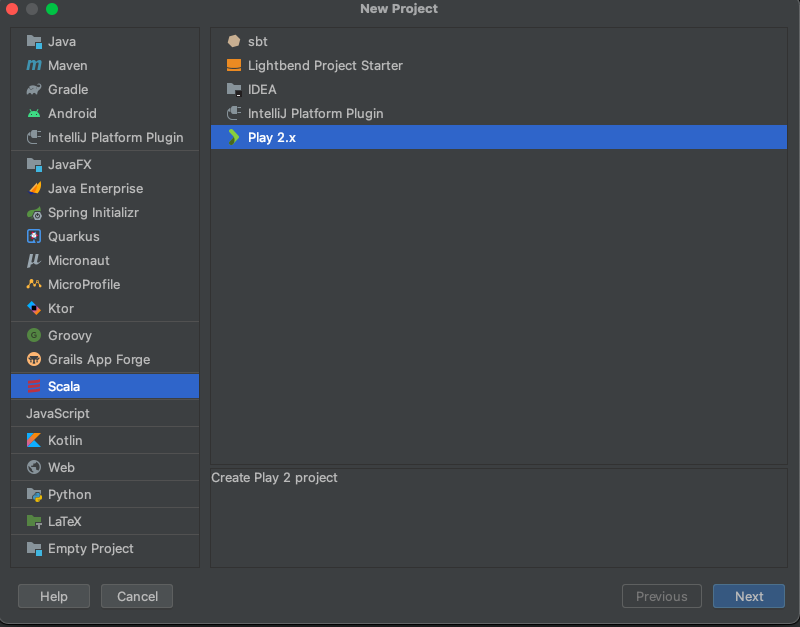
\includegraphics[width=10cm]{gfx/sbtplaysetup}
    \caption{SBT PlayFramework2.x setup screen 1}
    \label{fig:sbtplaysetupscreen1}
\end{figure}
Vervolgens zijn er een aantal dependencies aan het project toegevoegd:
\begin{lstlisting}[caption={build.sbt},label=lst:build.sbt]
name := "testPlayFramework"
version := "1.0"
lazy val `testplayframework` = (project in file(".")).enablePlugins(PlayScala)
resolvers += "Akka Snapshot Repository" at "https://repo.akka.io/snapshots/"
scalaVersion := "2.13.5"

libraryDependencies ++= Seq(jdbc, ehcache, ws, specs2 % Test, guice,
"com.typesafe.play" %% "play" % "2.8.8",
"com.typesafe.play" %% "play-json" % "2.9.2",
"com.typesafe.play" %% "play-test" % "2.8.8" % "test",
"org.scalatestplus.play" %% "scalatestplus-play" % "5.1.0" % "test",

"org.scalikejdbc" %% "scalikejdbc" % "3.5.0",
"com.h2database" % "h2" % "1.4.200",
"ch.qos.logback" % "logback-classic" % "1.2.3",
)

\end{lstlisting}
In deze snippet is te zien dat er een aantal bibliotheken zijn toegevoegd, in het project worden deze niet gebruikt, alleen maar als dependency om te kunnen scannen.


\subsection{setup SBT-Dependency Check}\label{subsec:setup-sbt-dependency-check}
Om SBT-dependency-check te kunnen gebruiken moet er een plugin worden toegvoegd. deze wordt toegevoegd aan de plugins.sbt in de project folder zoals hieronder te zien.
\begin{lstlisting}[caption={plugin.sbt.sbt},label=lst:plugin.sbt]
logLevel := Level.Warn

resolvers += "Typesafe repository" at "https://repo.typesafe.com/typesafe/releases/"

addSbtPlugin("com.typesafe.play" % "sbt-plugin" % "2.8.8")
addSbtPlugin("net.vonbuchholtz" % "sbt-dependency-check" % "3.2.0")


\end{lstlisting}
Op het moment dat de plugin vermeld staat in plugins.sbt dan heeft SBT de mogelijkheid om taken die in de plugin staat uit te voeren. Door de taak \texttt{sbt dependencyCheck} uit te voeren wordt er een rapport in HTML uitgegeven. Echter willen we een output in JSON waar we verder mee kunnen werken in de API.

in de build.sbt dienen we de volgende regel \texttt{dependencyCheckFormat := "JSON"} toe te voegen om een JSON bestand uit de tool te verkrijgen.

\subsection{resultaten}\label{subsec:SBTResultaten}
Het resultaat is een JSON bestand welke gegevens bevat van alle dependencies welke door de tool zijn geannalyseert in deze json worden ook alle kwetsbaarheden per dependency uiteengezet.


\section{NPM -audit voor Node/AngularProjecten}\label{sec:npm--audit-voor-node/angularprojecten}
Angular project opgezet middels de IntelliJ wizard.

\subsection{Opzetten van een Angular project}\label{subsec:opzetten-van-een-project-ang}

\subsection{setup NPM-audit}\label{subsec:setup-npm-audit}
NPM audit is al inbegrepen in de toolset van NPM dus kan ieder moment aangeroepen worden middels \texttt{npm -audit} als we een JSON output willen dienen we de glad \texttt{--json toe te voegen. }
Het probleem is alleen dat deze manier van werken geen artifact opleverd in een bestand maar alleen een screendump.
Door deze te "pipen" naar een bestand kunnen we de dump veilig stellen.
\subsection{resultaten}\label{subsec:ang-resultaten}
De resulataten van Json zijn ook in Json en goed te gebruiken om in een database te zetten.



\section{Test API}\label{sec:test-api}
De volgende stap om te kijken of er op een manier getriggerd kan worden wanneer een sbt wordt opgehaald.
